\subsection{Aspectes d'usabilitat considerats}

    \paragraph{}
    Les funcions de connexió i desconnexió, no requereixen gaires interaccions per part de l'usuari i per tant, no s'han pogut tractar gaires aspectes d'usabilitat. No obstant això, sí que s'ha volgut informar a l'usuari de què s'està esperant la seva identificació amb FamilySearch, quan aquest prem el botó d'identificació.

    Quan el pop up d'identificació amb FamilySearch és mostrat, el contingut de la pàgina \emph{login.html} s'esvaeix i apareix la imatge animada, mostrada a la figura~\ref{fig:fsLoginWait}. Aquesta imatge, indica que s'està esperant una interacció per part de l'usuari. Quan l'usuari acaba el procés d'identificació, aquest és redirigit de forma automàtica a la pàgina d'exemples o a la pàgina principal en cas d'error.

    \begin{figure}[h]
        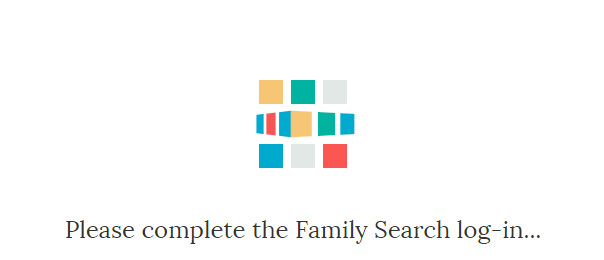
\includegraphics[scale=0.5]{11/01_loginLogout/02_waitingLogin}
        \centering
        \caption{Imatge animada mostrada mentre s'espera l'identificació de l'usuari}\label{fig:fsLoginWait}
    \end{figure}

    El segon aspecte d'usabilitat considerat, és que el botó de desconnectar-se només apareix, evidentment, si l'usuari es troba identificat.
